\subsection{LASSO}\label{apen:lasso}

LASSO is a categorized procedure within the set of penalized regressions. Penalized Least Squares is a punishment procedure that adds to the OLS regression a component that penalizes weak coefficients. The Penalty Least Squares estimator is obtained through

\begin{align*}
	\widehat{\boldsymbol{\beta}}(\lambda)=\underset{\boldsymbol{\beta} \in \mathcal{B}}{\arg \min }\left[\sum_{i=1}^n\left(Y_i-\boldsymbol{\beta}^{\prime} \boldsymbol{X}_i\right)^2+\sum_{j=1}^p p_\lambda\left(\left|\beta_j\right| ; \boldsymbol{\alpha}, \text { data }\right)\right]
\end{align*}

where $p_\lambda\left(\left|\beta_j\right| ; \boldsymbol{\alpha}, \text{data}\right)$ is a non-negative penalty function indexed by the regularization parameter $\lambda$ and could rely on both the data and additional hyperparameters. For example,

\begin{itemize}
	\item Ridge
	
	$p_\lambda\left(\left|\beta_j\right| ; \boldsymbol{\alpha}\right.$, data $)=\lambda\left|\beta_j\right|^2$
	\item LASSO
	
	$p_\lambda\left(\left|\beta_j\right| ; \boldsymbol{\alpha}\right.$, data $)=\lambda\left|\beta_j\right|$
	\item LASSO and Ridge combined
	
	$p_\lambda\left(\left|\beta_j\right| ; \boldsymbol{\alpha}\right.$, data $)=\alpha \lambda\left|\beta_j\right|+(1-\alpha) \lambda\left|\beta_j\right|^2$
\end{itemize}

The regularization parameter $\lambda$ controls the number of parameters in the model. If $\lambda = \infty$, then no parameters enter the model, and if $\lambda = 0$, then the parameters are simply OLS estimators.



% FIGURES
\newpage
\subsection{Figures}


\begin{figure}[H]
	\caption{Number of stocks in each Database}
	\centering
	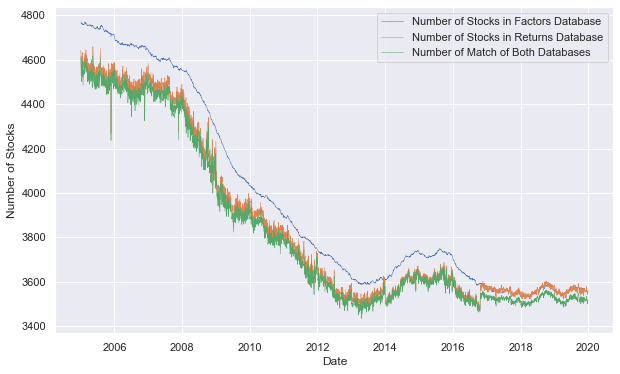
\includegraphics[scale=.73]{../../output/figures/match.png}
	\label{fig:match}
\end{figure}



\begin{figure}[H]
	\caption{Size Factor Returns Distribution}
	\centering
	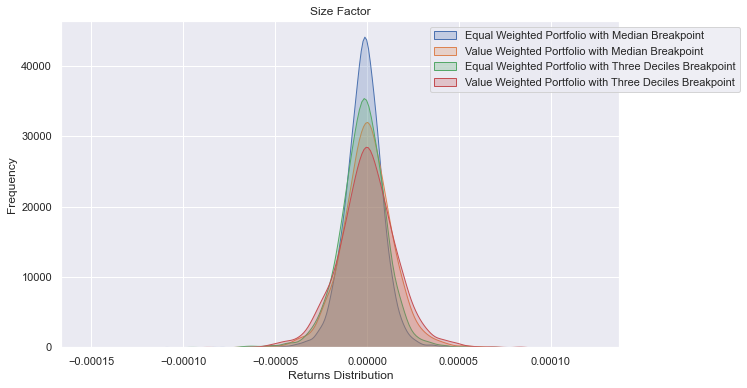
\includegraphics[scale=.63]{../../output/figures/size.png}
	\label{fig:size}
\end{figure}

\begin{figure}[H]
	\caption{Value (annual) Factor Returns Distribution}
	\centering
	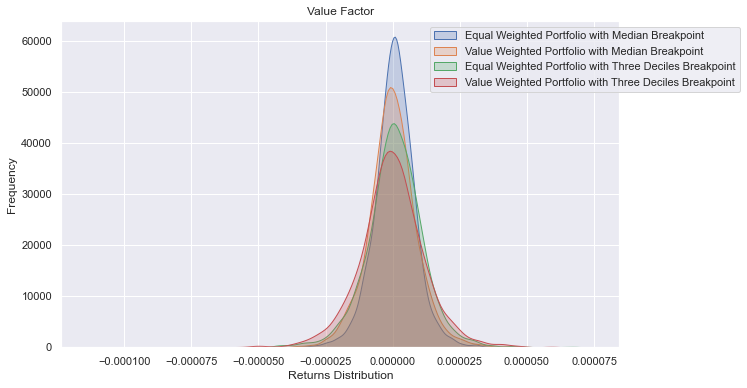
\includegraphics[scale=.63]{../../output/figures/value.png}
	\label{fig:value}
\end{figure}

\begin{figure}[H]
	\caption{Gross Profitability Factor Returns Distribution}
	\centering
	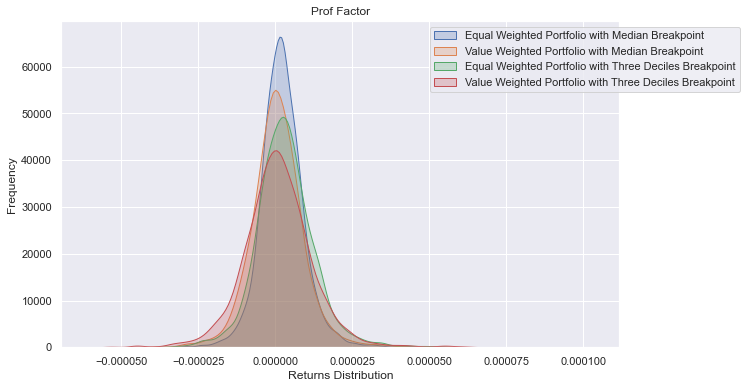
\includegraphics[scale=.63]{../../output/figures/prof.png}
	\label{fig:prof}
\end{figure}

\begin{figure}[H]
	\caption{Cash Flow Duration Factor Returns Distribution}
	\centering
	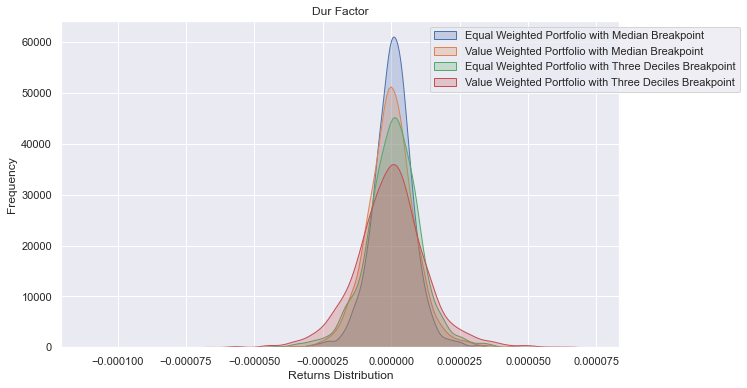
\includegraphics[scale=.63]{../../output/figures/dur.png}
	\label{fig:dur}
\end{figure}

\begin{figure}[H]
	\caption{Value-Profitability Factor Returns Distribution}
	\centering
	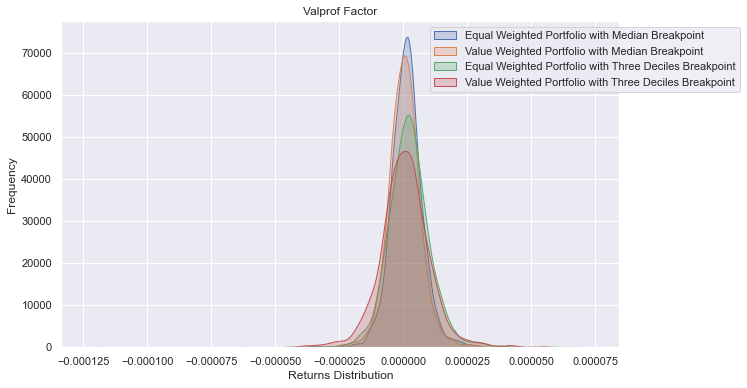
\includegraphics[scale=.63]{../../output/figures/valprof.png}
	\label{fig:valprof}
\end{figure}

\begin{figure}[H]
	\caption{Piotroski's F-score Factor Returns Distribution}
	\centering
	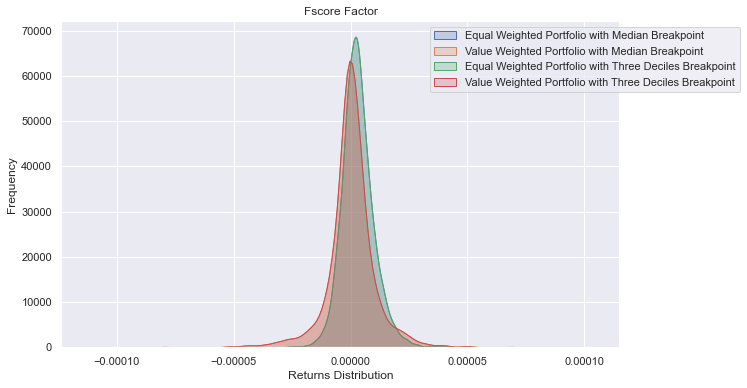
\includegraphics[scale=.63]{../../output/figures/fscore.png}
	\label{fig:fscore}
\end{figure}

\begin{figure}[H]
	\caption{Debit Issuance Factor Returns Distribution}
	\centering
	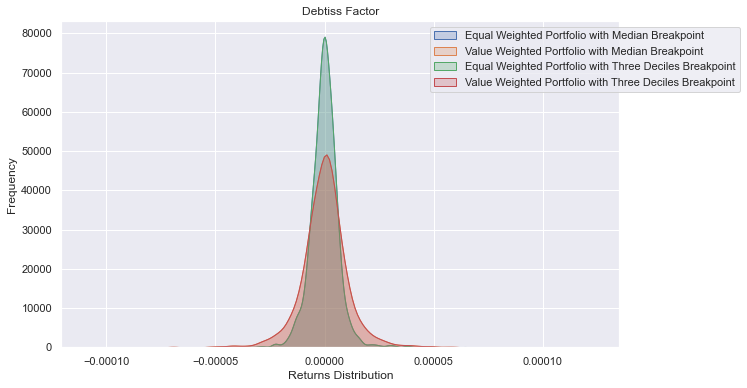
\includegraphics[scale=.63]{../../output/figures/debtiss.png}
	\label{fig:debtiss}
\end{figure}

\begin{figure}[H]
	\caption{Share Repurchases Factor Returns Distribution}
	\centering
	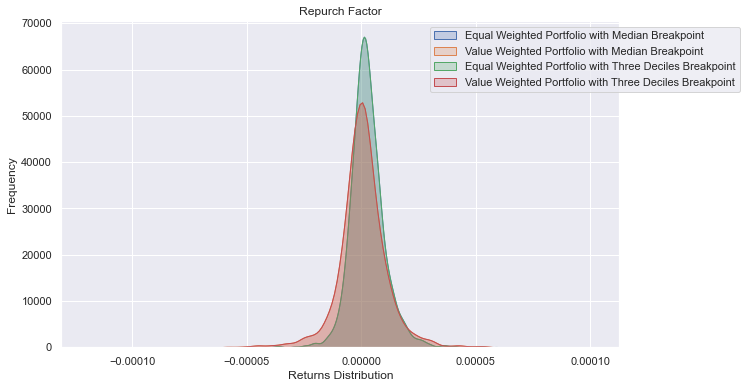
\includegraphics[scale=.63]{../../output/figures/repurch.png}
	\label{fig:repurch}
\end{figure}

\begin{figure}[H]
	\caption{Share Issuance (annual) Factor Returns Distribution}
	\centering
	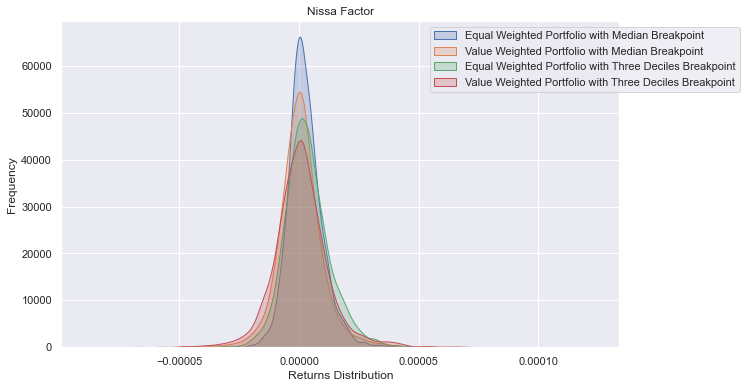
\includegraphics[scale=.63]{../../output/figures/nissa.png}
	\label{fig:nissa}
\end{figure}

\begin{figure}[H]
	\caption{Accruals Factor Returns Distribution}
	\centering
	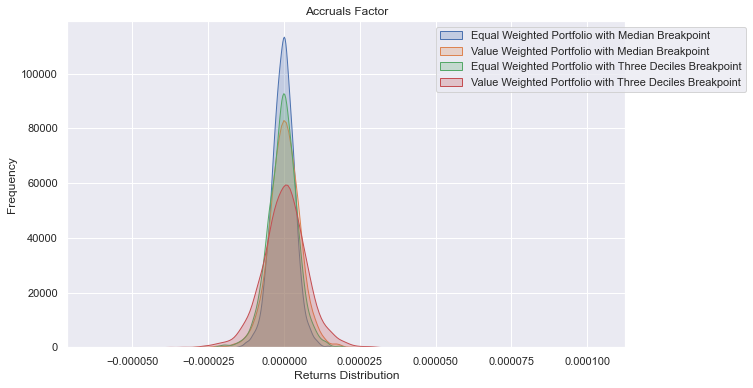
\includegraphics[scale=.63]{../../output/figures/accruals.png}
	\label{fig:accruals}
\end{figure}

\begin{figure}[H]
	\caption{Asset Growth Factor Returns Distribution}
	\centering
	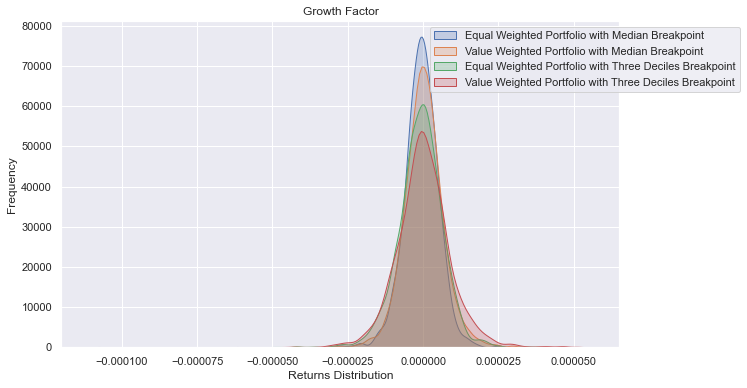
\includegraphics[scale=.63]{../../output/figures/growth.png}
	\label{fig:growth}
\end{figure}

\begin{figure}[H]
	\caption{Asset Turnover Factor Returns Distribution}
	\centering
	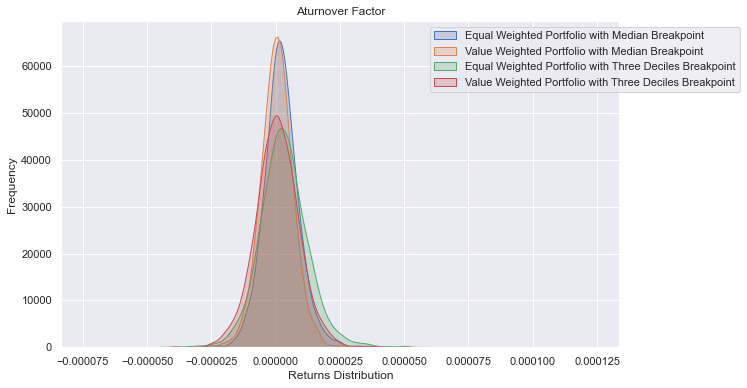
\includegraphics[scale=.63]{../../output/figures/aturnover.png}
	\label{fig:aturnover}
\end{figure}

\begin{figure}[H]
	\caption{Gross Margins Factor Returns Distribution}
	\centering
	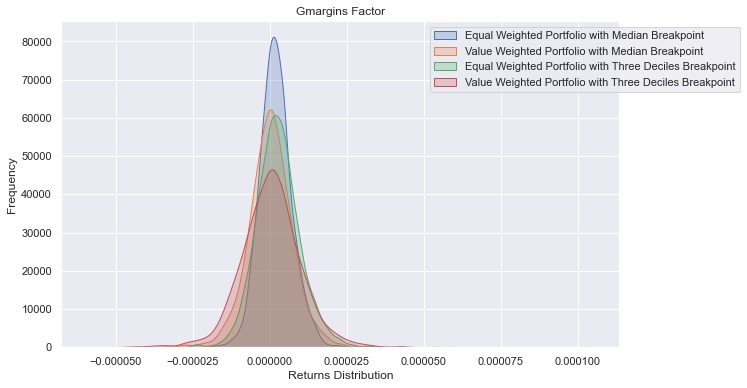
\includegraphics[scale=.63]{../../output/figures/gmargins.png}
	\label{fig:gmargins}
\end{figure}

\begin{figure}[H]
	\caption{Dividend Yield Factor Returns Distribution}
	\centering
	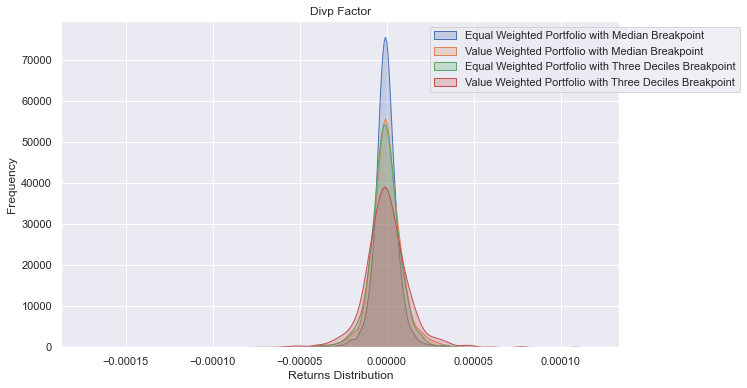
\includegraphics[scale=.63]{../../output/figures/divp.png}
	\label{fig:divp}
\end{figure}

\begin{figure}[H]
	\caption{Earnings/Price Factor Returns Distribution}
	\centering
	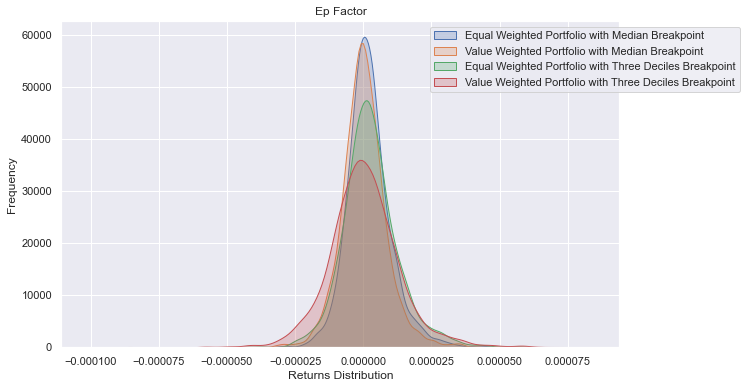
\includegraphics[scale=.63]{../../output/figures/ep.png}
	\label{fig:ep}
\end{figure}

\begin{figure}[H]
	\caption{Cash Flow / Market Value of Equity Factor Returns Distribution}
	\centering
	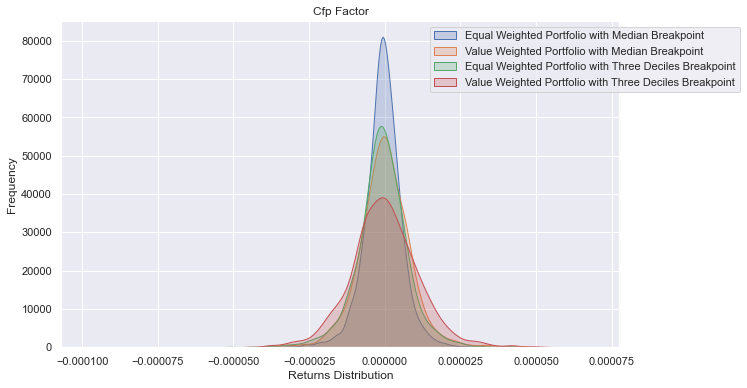
\includegraphics[scale=.63]{../../output/figures/cfp.png}
	\label{fig:cfp}
\end{figure}

\begin{figure}[H]
	\caption{Net Operating Assets Factor Returns Distribution}
	\centering
	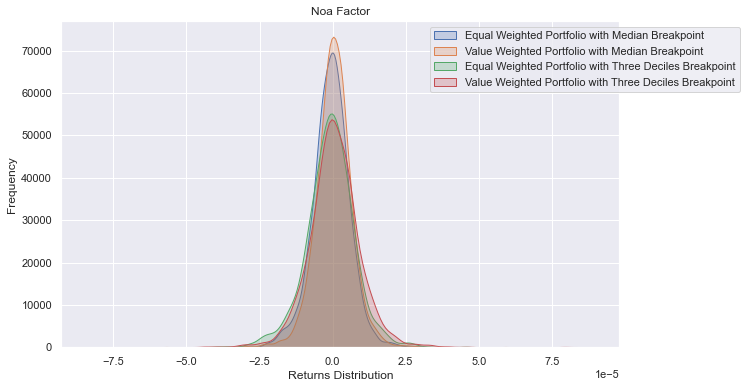
\includegraphics[scale=.63]{../../output/figures/noa.png}
	\label{fig:noa}
\end{figure}

\begin{figure}[H]
	\caption{Investment Factor Returns Distribution}
	\centering
	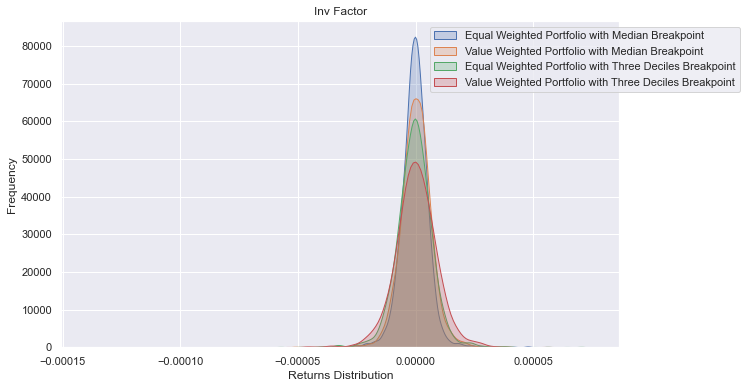
\includegraphics[scale=.63]{../../output/figures/inv.png}
	\label{fig:inv}
\end{figure}

\begin{figure}[H]
	\caption{Investment-to-Capital Factor Returns Distribution}
	\centering
	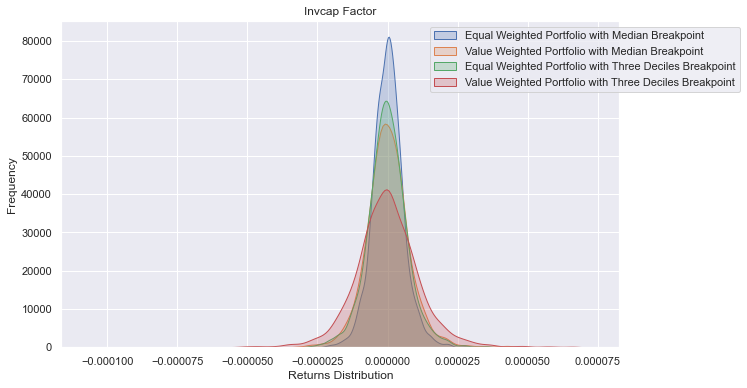
\includegraphics[scale=.63]{../../output/figures/invcap.png}
	\label{fig:invcap}
\end{figure}

\begin{figure}[H]
	\caption{Investment Growth Factor Returns Distribution}
	\centering
	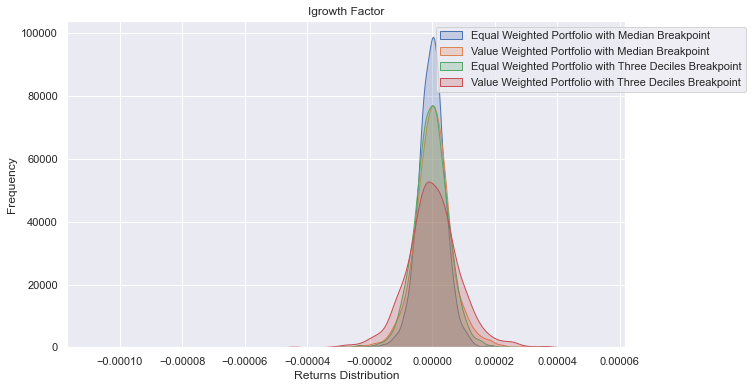
\includegraphics[scale=.63]{../../output/figures/igrowth.png}
	\label{fig:igrowth}
\end{figure}

\begin{figure}[H]
	\caption{Sales Growth Factor Returns Distribution}
	\centering
	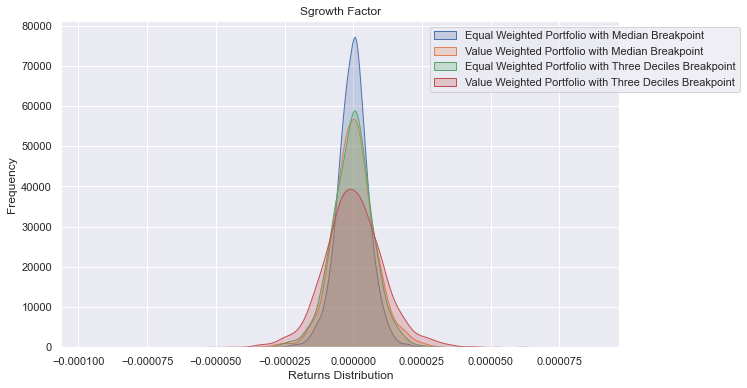
\includegraphics[scale=.63]{../../output/figures/sgrowth.png}
	\label{fig:sgrowth}
\end{figure}

\begin{figure}[H]
	\caption{Leverage Factor Returns Distribution}
	\centering
	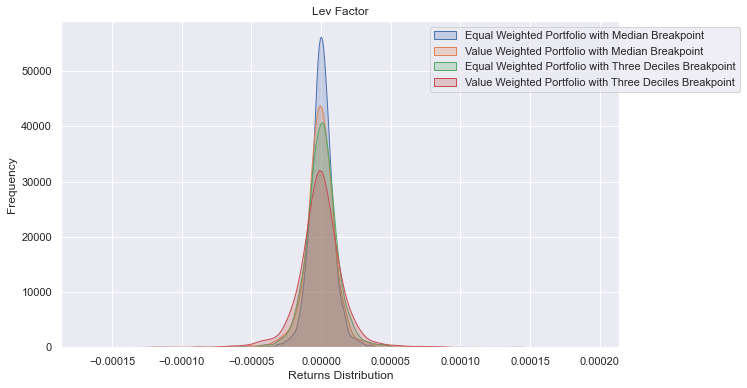
\includegraphics[scale=.63]{../../output/figures/lev.png}
	\label{fig:lev}
\end{figure}

\begin{figure}[H]
	\caption{Return on Assets (annual) Factor Returns Distribution}
	\centering
	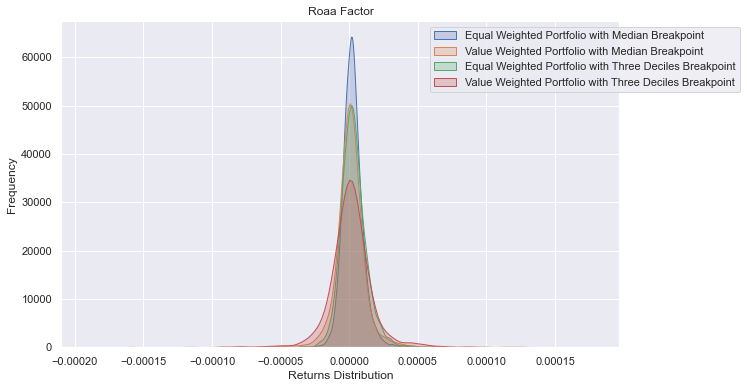
\includegraphics[scale=.63]{../../output/figures/roaa.png}
	\label{fig:roaa}
\end{figure}

\begin{figure}[H]
	\caption{Return on Equity (annual) Factor Returns Distribution}
	\centering
	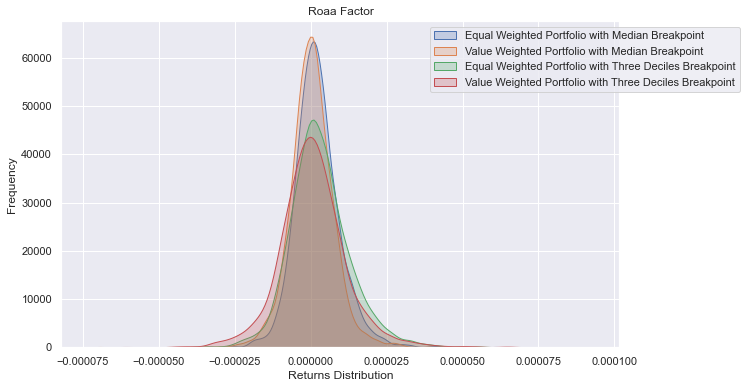
\includegraphics[scale=.63]{../../output/figures/roea.png}
	\label{fig:roea}
\end{figure}

\begin{figure}[H]
	\caption{Sales-to-Price Factor Returns Distribution}
	\centering
	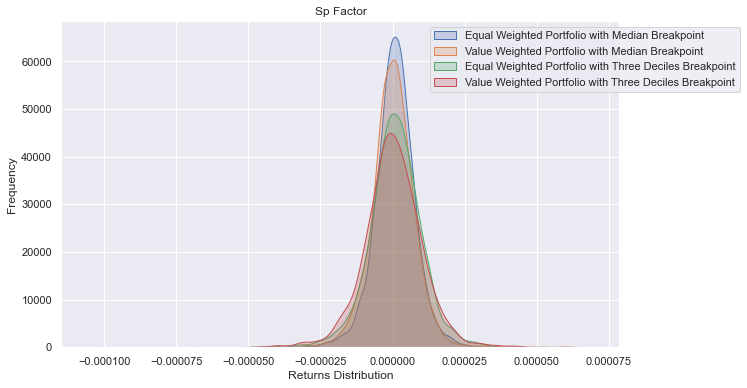
\includegraphics[scale=.63]{../../output/figures/sp.png}
	\label{fig:sp}
\end{figure}

\begin{figure}[H]
	\caption{Growth in LTNOA Factor Returns Distribution}
	\centering
	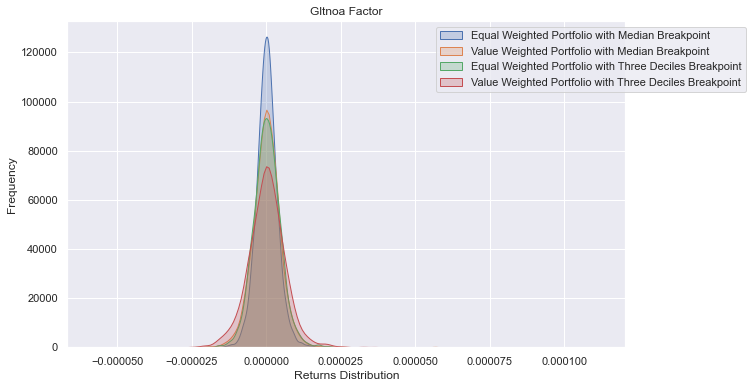
\includegraphics[scale=.63]{../../output/figures/gltnoa.png}
	\label{fig:gltnoa}
\end{figure}

%\begin{figure}[H]
%	\caption{Divg Factor Returns Distribution}
%	\centering
%	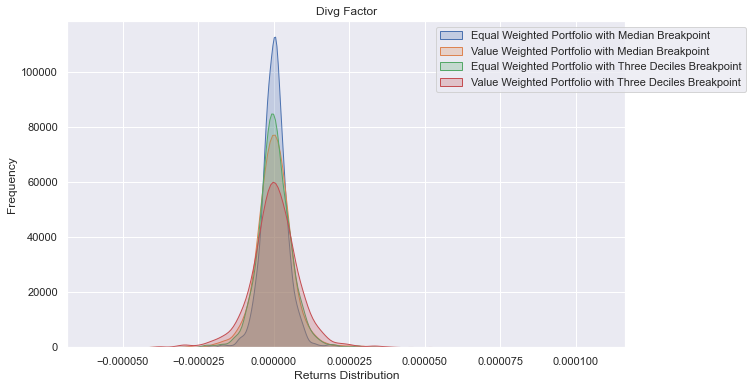
\includegraphics[scale=.63]{../../output/figures/divg.png}
%	\label{fig:divg}
%\end{figure}

%\begin{figure}[H]
%	\caption{Invaci Factor Returns Distribution}
%	\centering
%	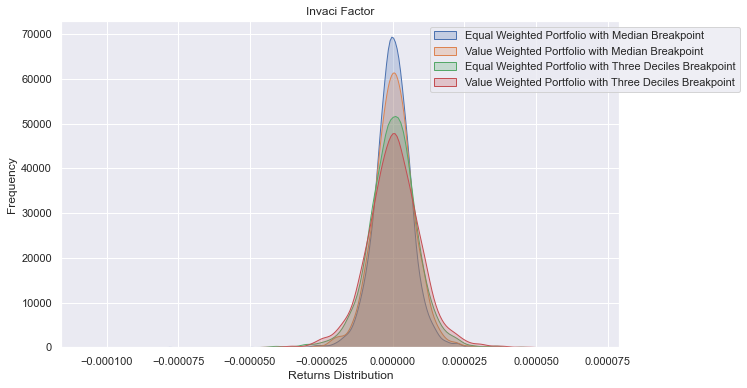
\includegraphics[scale=.63]{../../output/figures/invaci.png}
%	\label{fig:invaci}
%\end{figure}

\begin{figure}[H]
	\caption{Momentum (6m) Factor Returns Distribution}
	\centering
	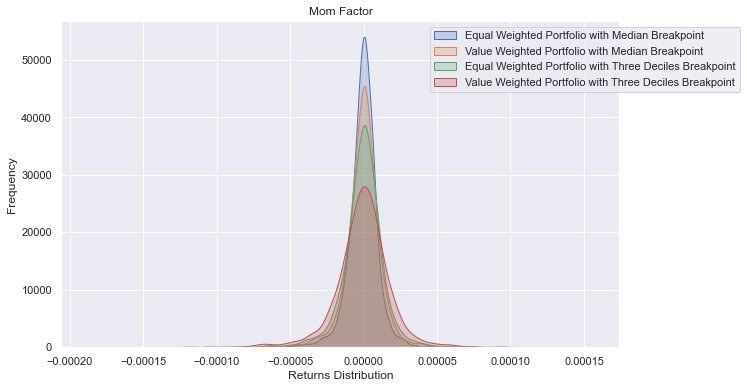
\includegraphics[scale=.63]{../../output/figures/mom.png}
	\label{fig:mom}
\end{figure}

\begin{figure}[H]
	\caption{Industry Momentum Factor Returns Distribution}
	\centering
	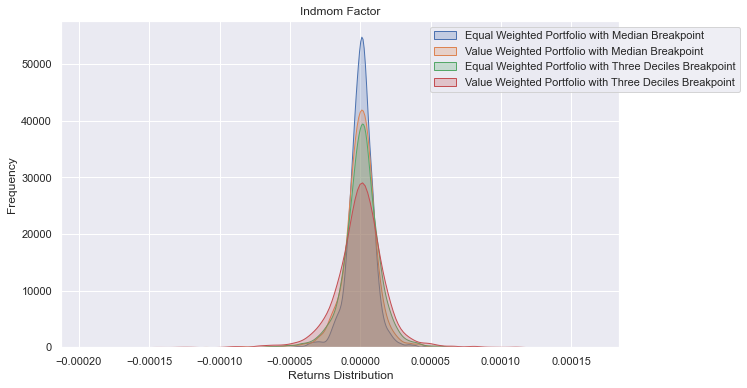
\includegraphics[scale=.63]{../../output/figures/indmom.png}
	\label{fig:indmom}
\end{figure}

\begin{figure}[H]
	\caption{Value-Momentum Factor Returns Distribution}
	\centering
	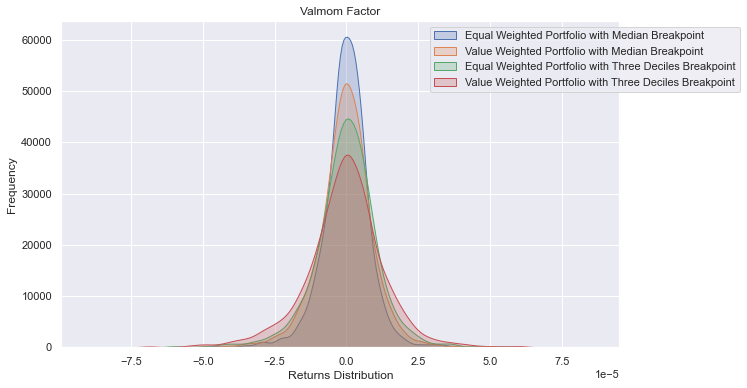
\includegraphics[scale=.63]{../../output/figures/valmom.png}
	\label{fig:valmom}
\end{figure}

\begin{figure}[H]
	\caption{Value-Momentum-Profitability Factor Returns Distribution}
	\centering
	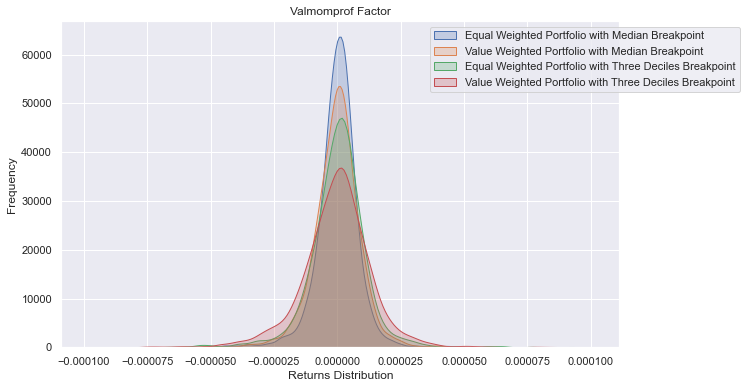
\includegraphics[scale=.63]{../../output/figures/valmomprof.png}
	\label{fig:valmomprof}
\end{figure}

\begin{figure}[H]
	\caption{Short Interest Factor Returns Distribution}
	\centering
	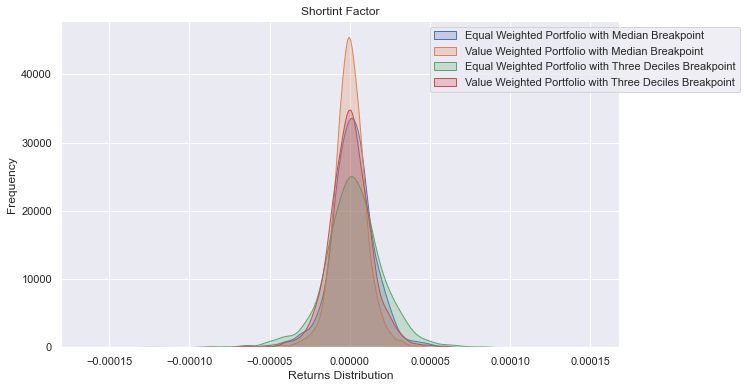
\includegraphics[scale=.63]{../../output/figures/shortint.png}
	\label{fig:shortint}
\end{figure}

\begin{figure}[H]
	\caption{Momentum (1 year) Factor Returns Distribution}
	\centering
	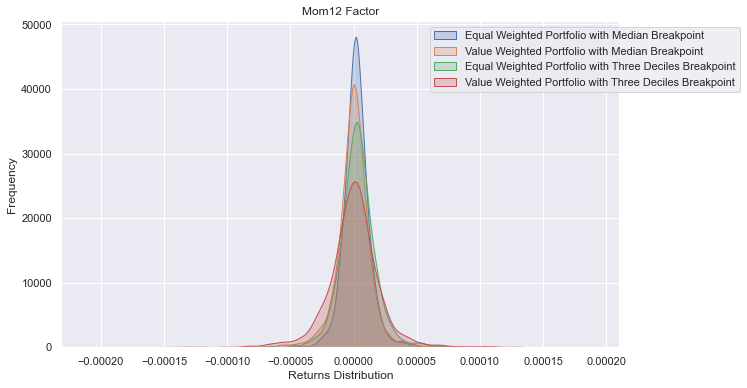
\includegraphics[scale=.63]{../../output/figures/mom12.png}
	\label{fig:mom12}
\end{figure}

\begin{figure}[H]
	\caption{Momentum-Reversal Factor Returns Distribution}
	\centering
	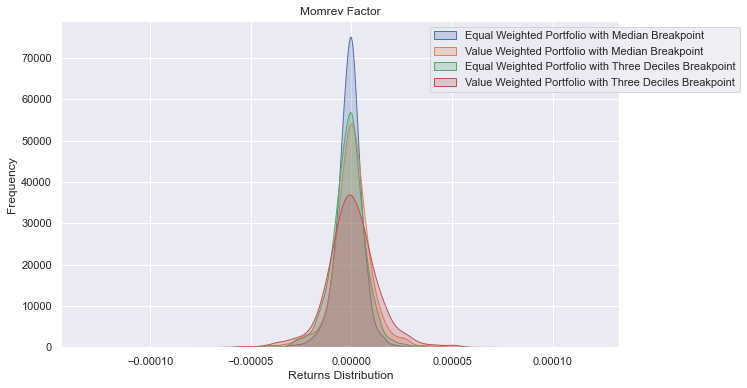
\includegraphics[scale=.63]{../../output/figures/momrev.png}
	\label{fig:momrev}
\end{figure}

\begin{figure}[H]
	\caption{Long-term Reversals Factor Returns Distribution}
	\centering
	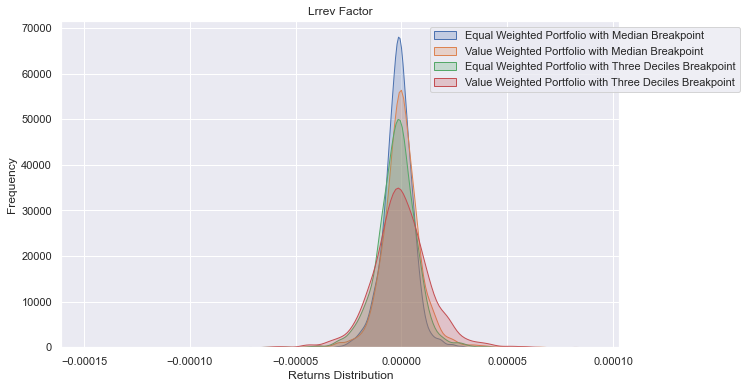
\includegraphics[scale=.63]{../../output/figures/lrrev.png}
	\label{fig:lrrev}
\end{figure}

\begin{figure}[H]
	\caption{Value (monthly) Factor Returns Distribution}
	\centering
	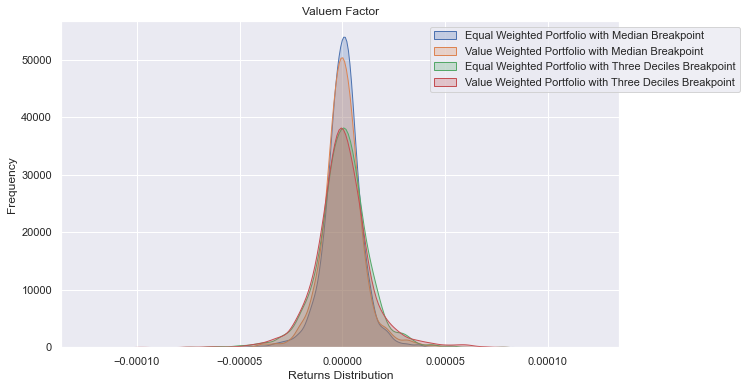
\includegraphics[scale=.63]{../../output/figures/valuem.png}
	\label{fig:valuem}
\end{figure}

\begin{figure}[H]
	\caption{Share Issuance (monthly) Factor Returns Distribution}
	\centering
	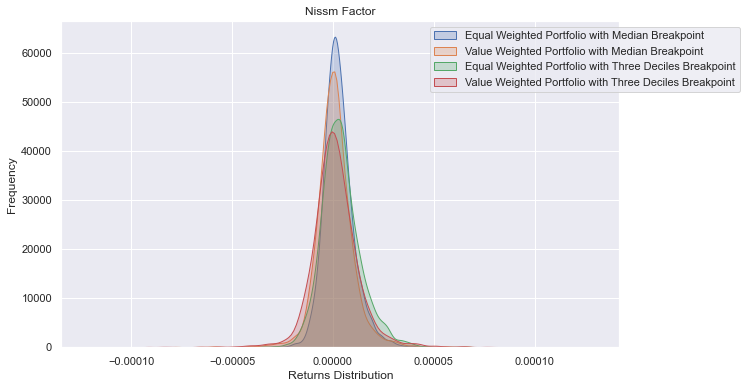
\includegraphics[scale=.63]{../../output/figures/nissm.png}
	\label{fig:nissm}
\end{figure}

\begin{figure}[H]
	\caption{PEAD (SUE) Factor Returns Distribution}
	\centering
	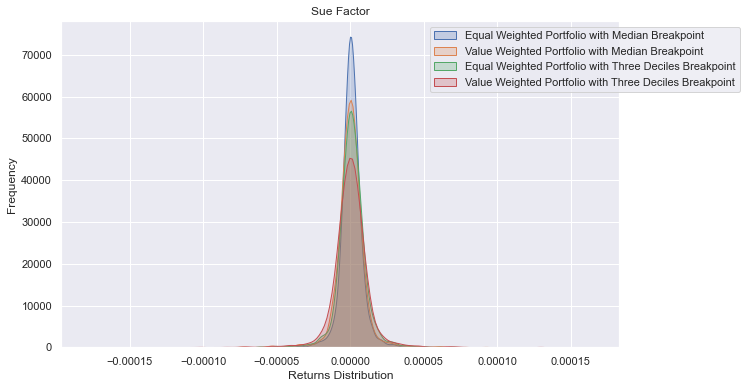
\includegraphics[scale=.63]{../../output/figures/sue.png}
	\label{fig:sue}
\end{figure}

\begin{figure}[H]
	\caption{Return on Book Equity Factor Returns Distribution}
	\centering
	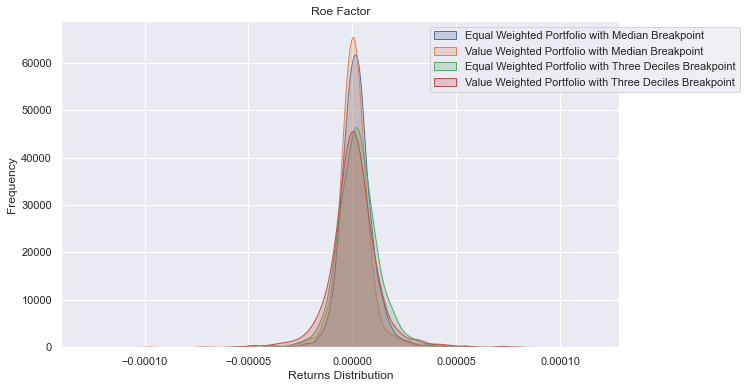
\includegraphics[scale=.63]{../../output/figures/roe.png}
	\label{fig:roe}
\end{figure}

\begin{figure}[H]
	\caption{Return on Market Equity Factor Returns Distribution}
	\centering
	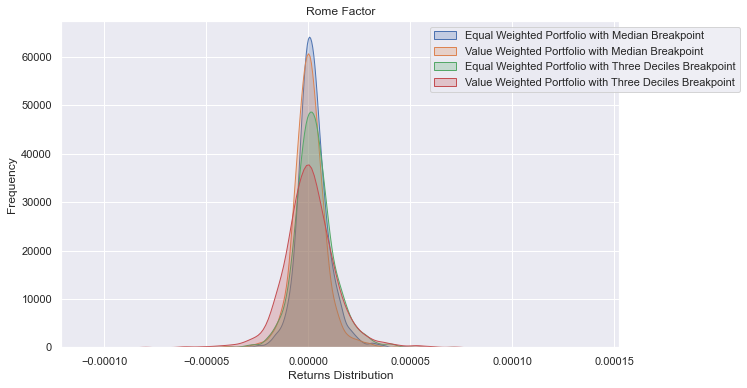
\includegraphics[scale=.63]{../../output/figures/rome.png}
	\label{fig:rome}
\end{figure}

\begin{figure}[H]
	\caption{Return on Assets Factor Returns Distribution}
	\centering
	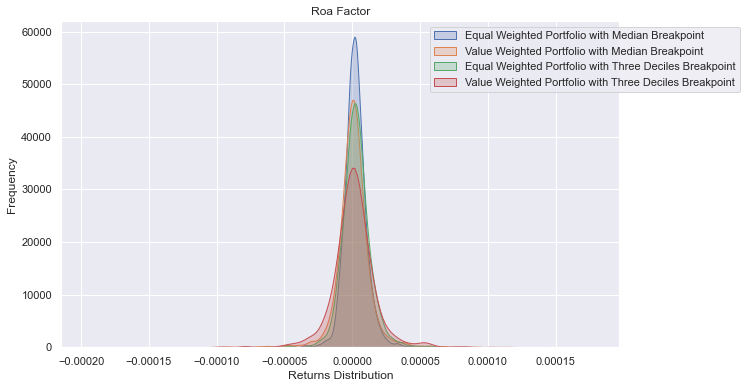
\includegraphics[scale=.63]{../../output/figures/roa.png}
	\label{fig:roa}
\end{figure}

\begin{figure}[H]
	\caption{Short-term Reversal Factor Returns Distribution}
	\centering
	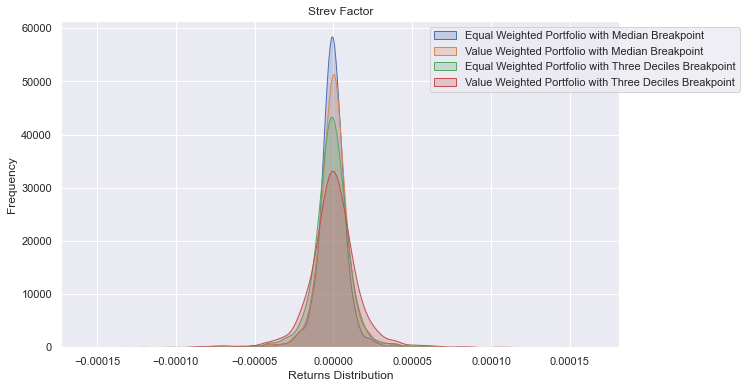
\includegraphics[scale=.63]{../../output/figures/strev.png}
	\label{fig:strev}
\end{figure}

\begin{figure}[H]
	\caption{Idiosyncratic Volatility Factor Returns Distribution}
	\centering
	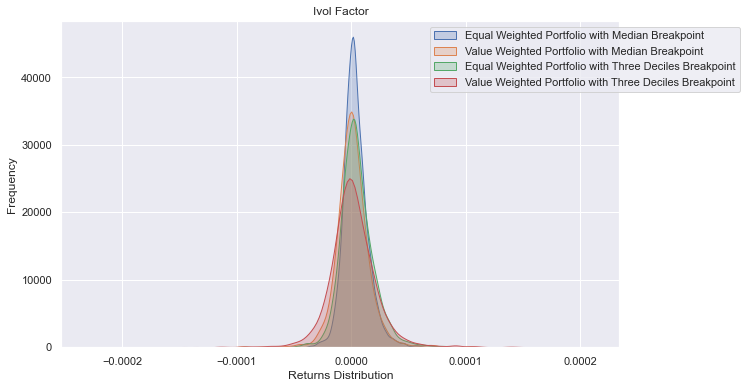
\includegraphics[scale=.63]{../../output/figures/ivol.png}
	\label{fig:ivol}
\end{figure}

\begin{figure}[H]
	\caption{Beta Arbitrage Factor Returns Distribution}
	\centering
	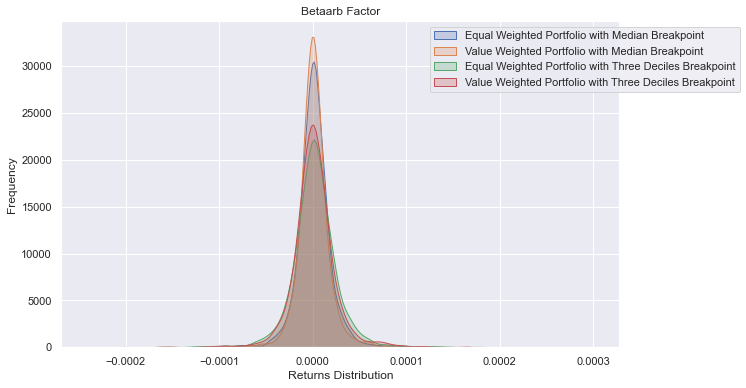
\includegraphics[scale=.63]{../../output/figures/betaarb.png}
	\label{fig:betaarb}
\end{figure}

\begin{figure}[H]
	\caption{Seasonality Factor Returns Distribution}
	\centering
	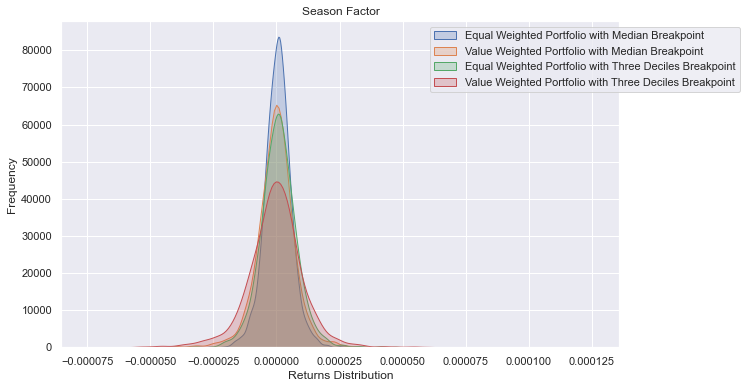
\includegraphics[scale=.63]{../../output/figures/season.png}
	\label{fig:season}
\end{figure}

\begin{figure}[H]
	\caption{Industry Relative Reversals Factor Returns Distribution}
	\centering
	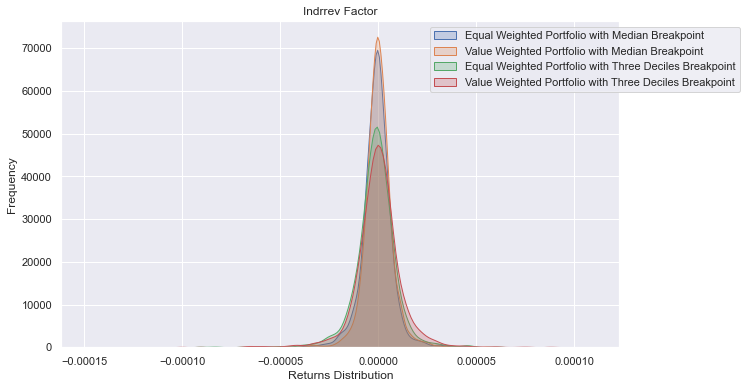
\includegraphics[scale=.63]{../../output/figures/indrrev.png}
	\label{fig:indrrev}
\end{figure}

\begin{figure}[H]
	\caption{Industry Relative Reversals (Low Volatility) Factor Returns Distribution}
	\centering
	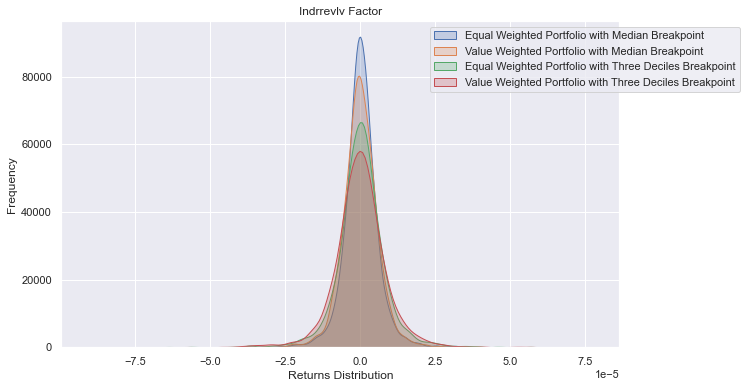
\includegraphics[scale=.63]{../../output/figures/indrrevlv.png}
	\label{fig:indrrevlv}
\end{figure}

\begin{figure}[H]
	\caption{Industry Momentum-Reversal Factor Returns Distribution}
	\centering
	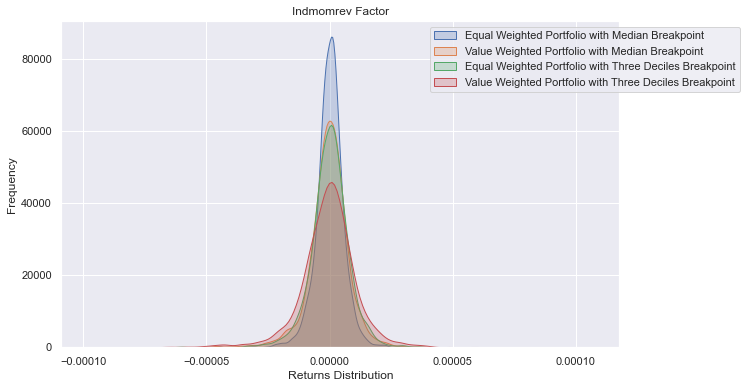
\includegraphics[scale=.63]{../../output/figures/indmomrev.png}
	\label{fig:indmomrev}
\end{figure}

\begin{figure}[H]
	\caption{Composite Issuance Factor Returns Distribution}
	\centering
	\includegraphics[scale=.63]{../../output/figures/ciss.png}
	\label{fig:ciss}
\end{figure}

\begin{figure}[H]
	\caption{Price Factor Returns Distribution}
	\centering
	\includegraphics[scale=.63]{../../output/figures/price.png}
	\label{fig:price}
\end{figure}

\begin{figure}[H]
	\caption{Firm Age Factor Returns Distribution}
	\centering
	\includegraphics[scale=.63]{../../output/figures/age.png}
	\label{fig:age}
\end{figure}

\begin{figure}[H]
	\caption{Share Volume Factor Returns Distribution}
	\centering
	\includegraphics[scale=.63]{../../output/figures/shvol.png}
	\label{fig:shvol}
\end{figure}

%\begin{figure}[H]
%	\caption{Exchsw Factor Returns Distribution}
%	\centering
%	\includegraphics[scale=.63]{../../output/figures/exchsw.png}
%	\label{fig:exchsw}
%\end{figure}
%
%\begin{figure}[H]
%	\caption{Ipo Factor Returns Distribution}
%	\centering
%	\includegraphics[scale=.63]{../../output/figures/ipo.png}
%	\label{fig:ipo}
%\end{figure}





% TABLES
%\newpage
%\subsection{Tables}
%
%\begin{table}[H]
%\caption{}
%\centering
%\begin{threeparttable}
%%\input{../../output/}
%\end{threeparttable}
%\label{tab:}
%\end{table}






%% PORTUGUESE VERSION
%
%O LASSO é um procedimento categorizado dentro do conjunto de regressões penalizadas. O Penalized Least Squares é um procedimento de estimação que adiciona ao OLS um componente que penaliza os coeficientes fracos. O estimador de Penalized Least Squares é obtido através
%
%\begin{align*}
%	\widehat{\boldsymbol{\beta}}(\lambda)=\underset{\boldsymbol{\beta} \in \mathcal{B}}{\arg \min }\left[\sum_{i=1}^n\left(Y_i-\boldsymbol{\beta}^{\prime} \boldsymbol{X}_i\right)^2+\sum_{j=1}^p p_\lambda\left(\left|\beta_j\right| ; \boldsymbol{\alpha}, \text { data }\right)\right]
%\end{align*}
%
%onde $p_\lambda\left(\left|\beta_j\right| ; \boldsymbol{\alpha}, \text{data}\right)$ é uma função penalidade não negativa indexada pelo parâmetro de regularização $\lambda$ e poderia depender tanto dos dados quanto de hiper-parâmetros adicionais. Por exemplo,
%
%\begin{itemize}
%	\item Ridge
%	
%	$p_\lambda\left(\left|\beta_j\right| ; \boldsymbol{\alpha}\right.$, data $)=\lambda\left|\beta_j\right|^2$
%	\item LASSO
%	
%	$p_\lambda\left(\left|\beta_j\right| ; \boldsymbol{\alpha}\right.$, data $)=\lambda\left|\beta_j\right|$
%	\item LASSO e Ridge combinado
%	
%	$p_\lambda\left(\left|\beta_j\right| ; \boldsymbol{\alpha}\right.$, data $)=\alpha \lambda\left|\beta_j\right|+(1-\alpha) \lambda\left|\beta_j\right|^2$
%\end{itemize}
%
%O parâmetro de regularização $\lambda$ controla o número de parâmetros no modelo. Se $\lambda = \infty$, então nenhum parâmetro entra no modelo, e se $\lambda = 0$, então os parâmetros são simplesmente estimadores OLS.

